\documentclass[11pt]{article}       % use "amsart" instead of "article" for AMSLaTeX format
\usepackage{geometry}                        % See geometry.pdf to learn the layout options. There are lots.


\geometry{a4paper}                   		% ... or a4paper or a5paper or ... 
%\geometry{landscape}                		% Activate for for rotated page geometry
%\usepackage[parfill]{parskip}    		% Activate to begin paragraphs with an empty line rather than an indent

\usepackage{caption}
\usepackage{float}
\usepackage{parskip}
\usepackage{amsmath}
\usepackage{graphicx}
\graphicspath{ {images/} }
				% Use pdf, png, jpg, or eps with pdflatex; use eps in DVI mode
								% TeX will automatically convert eps --> pdf in pdflatex	
\usepackage{amssymb}
\usepackage{hyperref}
\usepackage{subfig}
\usepackage{setspace}
\usepackage{listings}
\usepackage{caption}
%\onespacing

%\usepackage{fancyhdr} % Headers and footers
%\pagestyle{fancy} % All pages have headers and footers
\setlength{\headheight}{26pt}
\setlength\parindent{0pt} % sets indent to zero
\setlength{\parskip}{10pt}


\title{Statistical Analysis of Network Data  \\ Course by Eric D. Kolaczyk \\ \emph{Project paper: Comparison of community detection methods in Facebook social networks}}

\author{Alexandre Combessie\footnote{Mainly in charge of data loading, descriptive analysis, and similarity weighting. Email: \href{mailto:alexandre.combessie@ensae.fr}{alexandre.combessie@ensae.fr} }
  \and
  David Duong-Prunier\footnote{Mainly in charge of researching and implementing community detection methods. Email: \href{mailto:david.duong.prunier@ensae.fr}{david.duong.prunier@ensae.fr}}
  \and
    Ismail Machraoui\footnote{Mainly in charge of data loading, feature preparation and performance evaluation. Email: \href{mailto:ismail.machraoui@ensae.fr}{ismail.machraoui@ensae.fr}}
    }

\begin{document}

\maketitle
\begin{abstract}
This project paper intends to explore the characteristics of a sample of Facebook ego-networks and to compare the performance of several unsupervised community detection methods on this dataset. We implement 4 methods: Leading Eigenvector, Walktrap, Markov Cluster (MCL); and Hierarchical Clustering, which accounts for mixed community membership. We use Facebook profiles to compute a similarity measure between users and weigh the network edges accordingly. We compute the Balanced Error Rate to evaluate the performance of each method with respect to the real social circles. The MCL method outperforms the others although it does not allow for mixed membership. We also find that similarity weights significantly improve the performance of the Walktrap and Hierarchical Clustering methods.

\end{abstract}


\section{Introduction}

For this project paper, we chose to apply our new knowledge of Statistical Analysis of Network Data \cite{kolaczyk2009statistical, kolaczyk2014statistical} to a common topic of interest: social media. In particular, we decided to study Facebook, the most prominent social networking website with 1.55 billion monthly active users as of September 30, 2015 \cite{facebookstat}. We leveraged the vast literature on the subject, in particular \cite{leskovec2012learning, mcauley2014discovering}, and anonymized ego-network datasets made available on Kaggle \cite{dataset} by Jure Leskovec and Julian McAuley. 

Besides understanding the key characteristics of these ego-networks, our goal is to automatically identify the various social circles among one's Facebook friends, in an unsupervised way. Since we have the real social circles in our dataset, as labeled by the egos, we can compare our prediction with the truth, and evaluate the performance of each method. The topic of community detection is important for all social networks, and especially for Facebook, which does not require users to label their social circles, contrary to Google+. From our own personal experience as Facebook users, it can be difficult to manually sort out a long list of friends. Automatically detecting communities can help users save time, and improve the overall Facebook experience through a better curation of the news feed.


Our paper is organized as follows. In section \ref{datasetdescription}, we examine the data available and undertake some exploratory network characterization in order to have an overall idea of our ego-networks. In particular, we study our networks' order, size, degree distribution, centrality measures, and cohesion. We also analyze the Facebook profile data available on each user, and social circle labels given by the ego. Afterwards in section \ref{communitydetection}, we will describe the selected community detection methods from the associated literature, and illustrate it with our ego-networks. We will also describe how we can turn Facebook profile information into vertex attributes and weigh the network edges based on attributes similarity. In section \ref{conclusion} we will introduce our performance measure, the Balanced Error Rate, and explain how to compute it. Thus, we will run a performance comparison between our community detection methods, with or without similarity weights.

\section{Descriptive analysis of our dataset} \label{datasetdescription}

The dataset \cite{dataset} comprises of 110 ego-networks extracted from the online social network Facebook. Vertices are defined as users, i.e. the ego and his or her friends. Edges represent mutual friendship, with no information on the "nature" and "intensity" of the friendship relation, so the network is undirected and unweighted. Some user profile information is also available for each vertex, such as the user's name, hometown, schools, and employers (past and present). All data has been anonymized, and there is no way to relate each network with each other. 

Besides, for all ego-networks, we have labels given by the ego user for the friends in their social circles. However, not all users have labels, as the ego users have provided partial information. Finally, in order to evaluate the performance of our community detection models, we have been provided the ground-truth circles, or might we say the "real" human-labeled circles, supplied by the ego users, for 60 ego-networks (not all of the 110).


\newpage
\subsection{Visualization} \label{viz}
In the next figure, we have plotted a sample of 4 ego-networks. We see that the order (number of vertices) and size (number of edges) of the network varies, with sparse and dense networks. As emphasized by the Fruchterman-Reingold layout, communities tend to appear visually. 

\begin{figure}[H]
\centering
  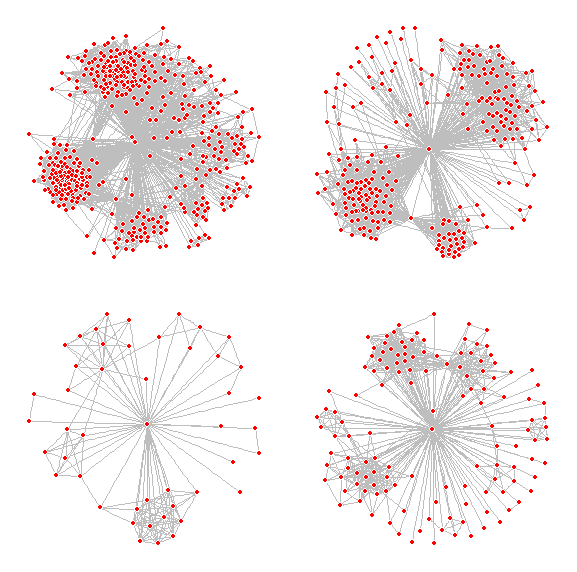
\includegraphics[width=0.7\linewidth]{viz4graph.png}
    \caption{Visualizations of a sample of networks, with the ego included}
\end{figure}

Note that we have included the ego for visualization purposes, but from now in this section, we will exclude the ego from our analysis, to facilitate the interpretation.

\subsection{Network order and size} \label{ordersize}

To better understand the characteristics of these ego-networks, we studied the distribution of the order and size of these networks (ego excluded). Here, order is simply the number of friends of the ego, and can be interpreted as a measure of sociability. Size is the number of friendship relations between friends of the ego. It is hard to interpret it in terms of network cohesion as studied in subsection \ref{networkcohesion}.

\begin{figure}[H]
\centering
  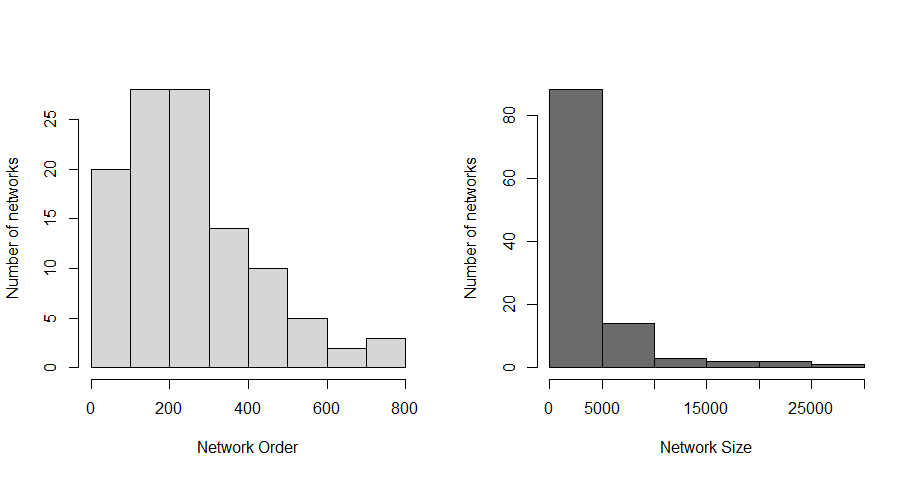
\includegraphics[width=\linewidth]{SizeOrderDistribution.png}
    \caption{Distribution of the order and size of all 110 networks, without the ego}
\end{figure}

\begin{table}[ht]
\centering
\begin{tabular}{rrr}
  \hline
 & Order & Size \\ 
  \hline
Minimum & 12 & 14 \\ 
  1st Quartile & 119 & 670 \\ 
  Median & 215 & 1686 \\ 
  Mean & 251 & 3388 \\ 
  3rd Quartile & 338 & 4129 \\ 
  Maximum & 781 & 25290 \\ 
   \hline
\end{tabular}
\caption{Summary statistics on the order and size of networks}
\end{table}

On average in our sample, an ego has 251 friends. The sample of 'egos' considered is relatively diverse, from a seemingly 'solitary ego' with 12 friends to a 'socially active' one with 781 friends. The order distribution is relatively smooth (Skewness of 1.10, Gini of 0.37), with a visually linear decay.

As for network size, the distribution is more skewed and unequal (Skewness of 2.74, Gini of 0.60), with a visually exponential decay.

\newpage

\subsection{Degree distribution} \label{degreedistribution}

To better characterize our sample of networks, we will study its degree distribution\footnote{Since the networks are unweighted, degree is equal to strength.}, i.e. the number of mutual friends with the ego for a given user. It can be interpreted in terms of "sociability" or "importance" of each user \emph{within} the network induced by friendship with the ego. Since each of our networks is only a sampled subgraph of the complete Facebook graph, it is a poor measure of real sociability or importance. To take an example, a popular user could have no mutual friends with the ego but still have a large group of friends not captured in the dataset. Therefore, we will be careful not to over-interpret this measure.

\begin{figure}[H]
\centering
\begin{minipage}[b]{0.55\linewidth}
\vspace{0pt}
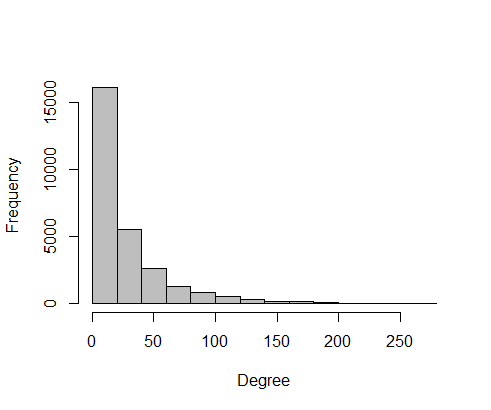
\includegraphics[width=\linewidth]{degreedistribution.png}
\caption{Degree distribution for all networks combined}
\end{minipage}
\hspace{0.5cm}
\begin{minipage}[b]{0.35\linewidth}
\captionsetup{type=table}
\centering
\begin{tabular}[b]{rr}
  \hline
 & Degree \\ 
  \hline
Minimum & 0 \\ 
  1st Quartile & 6 \\ 
  Median & 16 \\ 
  Mean & 27 \\ 
  3rd Quartile & 35\\ 
  Maximum & 276 \\ 
   \hline
\end{tabular}
\vspace{1.8cm}
\caption{Summary statistics on the degree distribution}
\end{minipage}
\end{figure}

On average for all networks combined, a user has 27 mutual friends with the ego. We see that the degree distribution is skewed and unequal (Skewness of 2.34, Gini of 0.57). As studied in many empirical works on social and information networks, our degree distribution seems to follow a power law \cite{clauset2009power, girvan2002community,ugander2011anatomy}. To verify it, we can apply a very simple Ordinary Least Squares model\footnote{It is only a first naive step, as more robust approaches exist today, such as maximum-likelihood fitting with goodness-of-fit tests based on the Kolmogorov Smirnov statistic and likelihood ratio \cite{clauset2009power}.}.    

\begin{figure}[H]
\centering
\begin{minipage}[b]{0.45\linewidth}
\vspace{0pt}
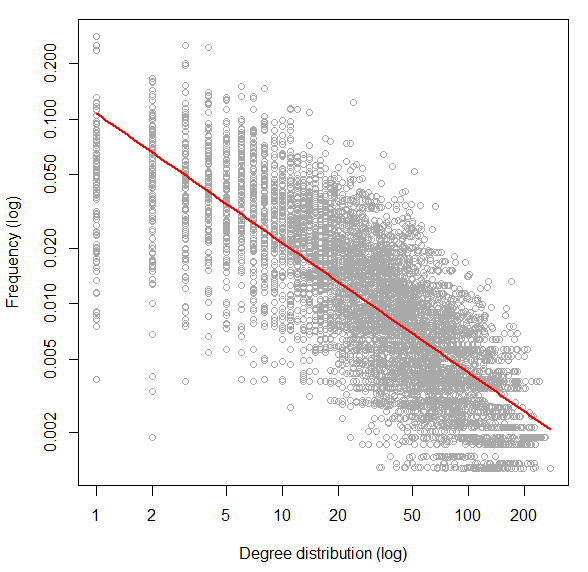
\includegraphics[width=\linewidth]{DegreePowerLaw.png}
\caption{Degree distribution for all networks combined, fitted to a power law}
\end{minipage}
\hspace{0.5cm}
\begin{minipage}[b]{0.45\linewidth}
\captionsetup{type=table}
\centering

\footnotesize
\begin{tabular}{@{\extracolsep{5pt}}lc} 
\\[-1.8ex]\hline 
\hline \\[-1.8ex] 
 & \multicolumn{1}{c}{\textit{Dependent variable:}} \\ 
\cline{2-2} 
\\[-1.8ex] & log(frequency) \\ 
\hline \\[-1.8ex] 
 log(degree) & $-$0.701$^{***}$ \\ 
  & (0.008) \\ 
  Constant & $-$2.238$^{***}$ \\ 
  & (0.027) \\ 
 \hline \\[-1.8ex] 
Observations & 6,034 \\ 
R$^{2}$ & 0.586 \\ 
Adjusted R$^{2}$ & 0.585 \\ 
Res. Std. Error & 0.660 (df = 6032) \\ 
F Statistic & 8,522.404$^{***}$ (df = 1; 6032) \\ 
\hline 
\hline \\[-1.8ex] 
\textit{Note:}  & \multicolumn{1}{r}{$^{*}$p$<$0.1; $^{**}$p$<$0.05; $^{***}$p$<$0.01} \\ 
\end{tabular} 

\vspace{0.7cm}
\caption{Summary of the OLS regression statistics}
\end{minipage}
\end{figure}

We see that the OLS regression coefficients are statistically significant at 99\%, provided the OLS normal assumptions are verified. However, to test the correct specification, we would need more in-depth models.

\subsection{Network centrality} \label{networkcentrality}

This is close to the previous section \ref{degreedistribution} on degree distribution. However, we will refrain from studying centrality in terms of flow of information in the network, because the ego-networks only offer a very incomplete view of the overall Facebook graph. In our dataset, centrality measures can only be interpreted as the relative social importance of the user strictly within the group of friends of the ego. 

For all networks combined, we can plot the distribution of several classic centrality measures: Closeness, Betweenness, and Eigenvector. The distribution of these measures being very skewed and unequal (see table below), we have plotted the distributions in log scale. We note that Eigenvector centrality produces a less skewed distribution.

\begin{table}[ht]
\centering
\begin{tabular}{rrr}
  \hline
 & Skewness & Gini \\ 
  \hline
Closeness Centrality & 16.72 & 0.63 \\ 
  Betweenness Centrality & 27.57 & 0.86 \\ 
  Eigenvector Centrality & 1.61 & 0.37 \\ 
   \hline
\end{tabular}
\caption{Skewness and Gini index of centrality distributions}
\end{table}

\begin{figure}[H]
\centering
  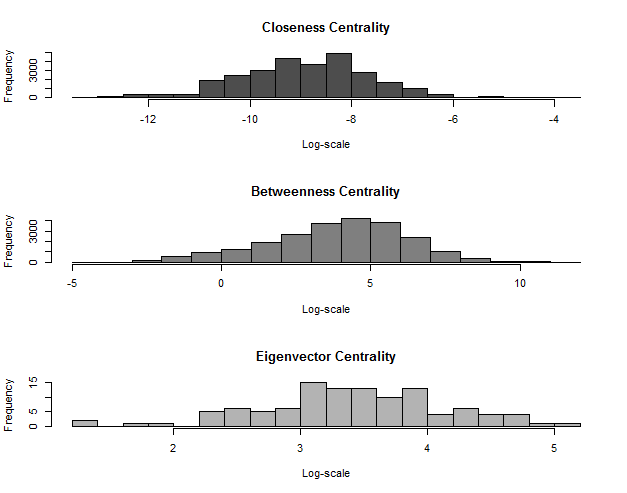
\includegraphics[width=0.8\linewidth]{centrality.png}
    \caption{Centrality distributions for all networks combined}
\end{figure}

The skewed nature of these distributions could be interpreted as the fact that people have only a few "important friends" within a larger group of "acquaintances", who are less central in the ego-network.

\subsection{Network cohesion} \label{networkcohesion}
To further study the subject mentioned above, it is interesting to study our networks in terms of cohesion: how dense are the networks? Are there a lot of "solitary nodes" with no mutual friends? How many vertices are in the largest cliques?

To answer these questions, we will study several indicators:
\begin{itemize}
  \item Density of each network, measured by $\frac{|E|}{|V|(|V|-1)/2}$
  \item Ratio of the giant component order on the total order, for each network: $\frac{|E_{giant}|}{|E_{total}|}$
  \item Distribution of order of components, for all networks combined
  \item Order of the largest cliques of each network
\end{itemize}

\newpage
\begin{figure}[H]
\centering
\begin{minipage}[b]{0.45\linewidth}
\vspace{0pt}
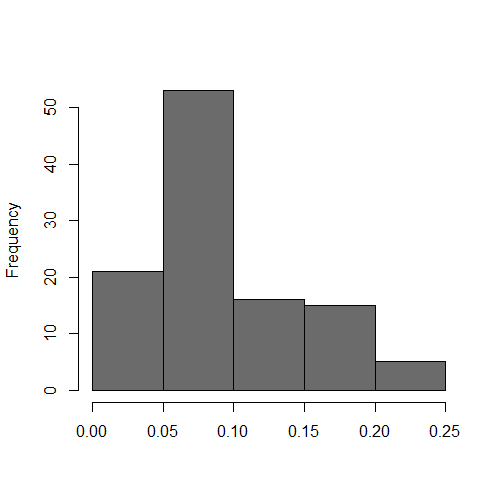
\includegraphics[width=\linewidth]{densitydist.png}
\caption{Distribution of the density of each network}
\end{minipage}
\hspace{0.5cm}
\begin{minipage}[b]{0.45\linewidth}
\centering
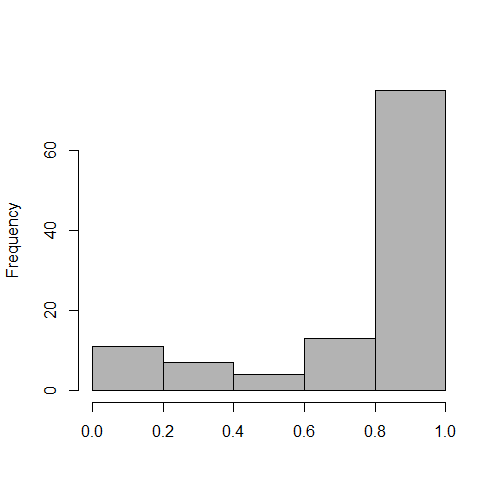
\includegraphics[width=\linewidth]{ratiocomponent.png}
\caption{Distribution of the ratio of order of the giant component}
\end{minipage}
\end{figure}

We see that the networks are not very dense (mean density of 9.3\%), and that the giant component represents the majority of the network (average of 76.5\% of the total order of each network). Thus the large majority of friends of the ego are part of a subgraph of mutual friends.

\begin{figure}[H]
\centering
  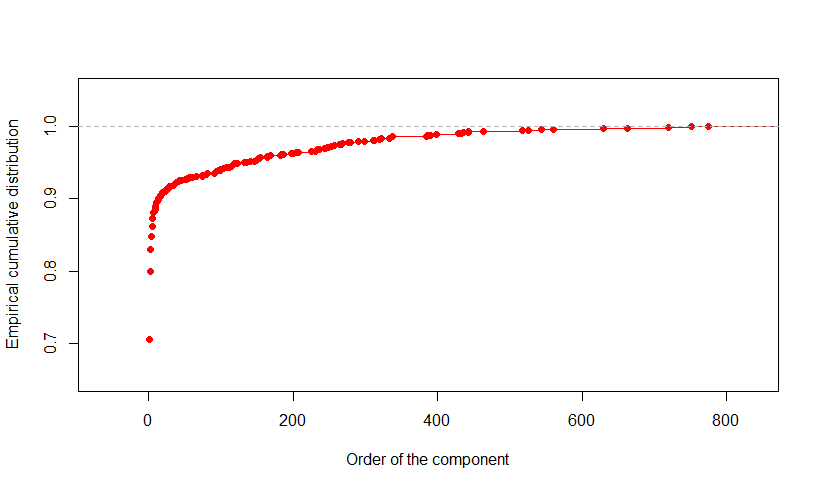
\includegraphics[width=0.8\linewidth]{componentecdf.png}
    \caption{Empirical cumulative distribution of components' order for all networks}
\end{figure}

As shown in the figure above, the distribution is skewed: atomic components represent 70.5\% of the count of components, but only 3.5\% of the total order of all networks.

\newpage

Finally, we will study the distribution of order of the largest cliques.

\begin{figure}[H]
\centering
\begin{minipage}[b]{0.47\linewidth}
\vspace{0pt}
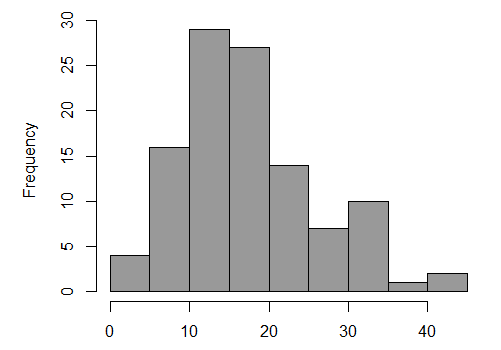
\includegraphics[width=\linewidth]{largestclique.png}
\caption{Distribution of order of the largest cliques in each network}
\end{minipage}
\hspace{0.5cm}
\begin{minipage}[b]{0.45\linewidth}
\captionsetup{type=table}
\centering
\begin{tabular}[b]{rr}
  \hline
 & Order \\ 
  \hline
Minimum & 4.0 \\ 
  1st Quartile & 12.0 \\ 
  Median & 16.5 \\ 
  Mean & 18.3 \\ 
  3rd Quartile & 23.0 \\ 
  Maximum & 42.0 \\ 
   \hline
\end{tabular}
\vspace{0.8cm}
\caption{Summary statistics on the largest cliques' orders}
\end{minipage}
\end{figure}

We see that the largest clique encompasses on average 18 friends, which can  be interpreted as the size of the group of "close friends" of the ego. However, the interpretation of "close friends" in this case is not the same as in section \ref{networkcentrality} on centrality.



\subsection{Feature completion} \label{featurecompletion}
In addition to the ego-networks, we have features from the Facebook profiles of each ego and friends. We flattened this feature data, which was originally under a tree format, to build a set of 56 vertex attributes\footnote{When considering only "name" and not "id" types of features, the number is reduced to 36.}. However, not all attributes were filled by the users: the ratio of completion of all features for a given network is low. There is more than 50\% of incomplete data for each network.

\begin{figure}[H]
\centering
\begin{minipage}[b]{0.47\linewidth}
\vspace{0pt}
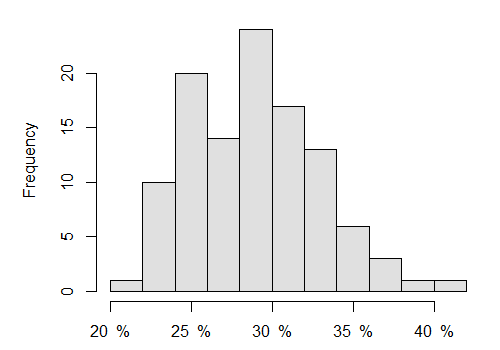
\includegraphics[width=\linewidth]{completion.png}
\caption{Distribution of the ratio of completion of all features by network}
\end{minipage}
\hspace{0.5cm}
\begin{minipage}[b]{0.45\linewidth}
\captionsetup{type=table}
\centering
\begin{tabular}[b]{rr}
  \hline
 & Ratio \\ 
  \hline
Minimum & 20.9\% \\ 
  1st Quartile & 25.6\% \\ 
  Median & 29.0\% \\ 
  Mean & 28.9\% \\ 
  3rd Quartile & 31.3\% \\ 
  Maximum & 41.2\% \\ 
   \hline
\end{tabular}
\vspace{0.8cm}
\caption{Summary statistics on the ratio of completion}
\end{minipage}
\end{figure}

\newpage
But the ratio of completion depends a lot on the features considered. Almost all users give their locale, name, gender and birthday information ; whereas very little information is available on the users' religion, political views, and work projects.


\begin{figure}[H]
\centering
  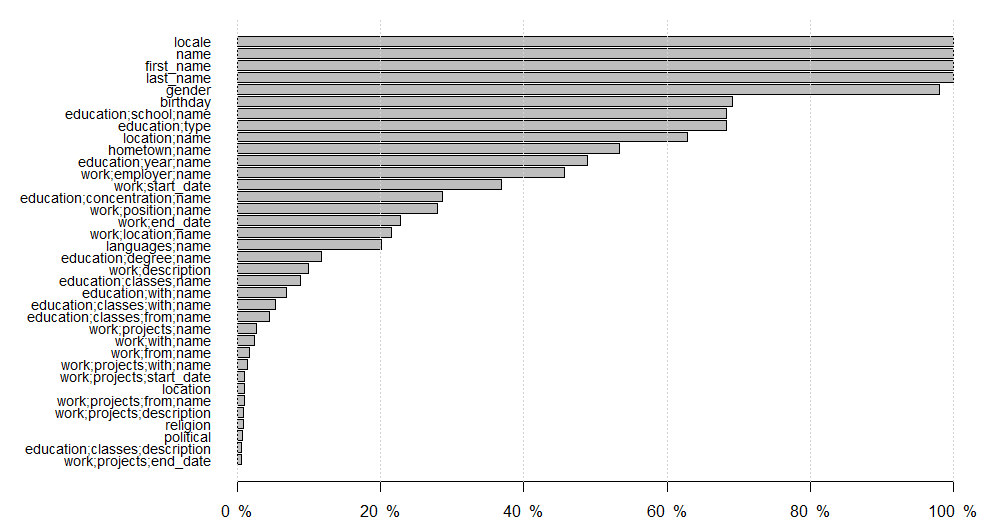
\includegraphics[width=\linewidth]{featurecompletion.png}
    \caption{Percentage of completion by feature, for all networks combined}
\end{figure}

\subsection{Analyzing user-labeled social circles} \label{socialcirclelabels}
Based on social circle training data we have on 60 ego-networks, we can answer several questions: How many circles to consider? How many friends does a circle contain? Does everyone belong to a circle? Is there a lot of overlap between circles?

\begin{figure}[H]
\centering
\begin{minipage}[b]{0.47\linewidth}
\vspace{0pt}
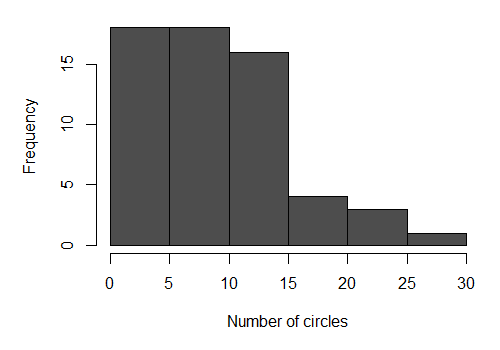
\includegraphics[width=\linewidth]{numcircles.png}
\caption{Distribution of the number of circles per ego}
\end{minipage}
\hspace{0.5cm}
\begin{minipage}[b]{0.47\linewidth}
\centering
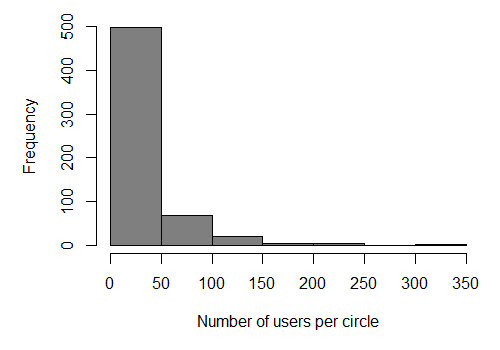
\includegraphics[width=\linewidth]{userpercircle.png}
\caption{Distribution of the number of users per circle for all networks combined}
\end{minipage}
\end{figure}
\newpage

From the previous figures, we see that the number of circles per ego is relatively uniform. It is less so for the distribution of number of users per circle. On average, each ego has defined 10 social circles, with 29 users per circle.

We also see that our training data is well labeled: on average in each ego-network, 80\% of users have been labeled to a social circle. Finally, the phenomenon of mixed membership is very important: 37\% of users are part of 2 or more social circles. We will need to take this into account in section \ref{communitydetection} on Community Detection.

\begin{figure}[H]
\centering
\begin{minipage}[b]{0.47\linewidth}
\vspace{0pt}
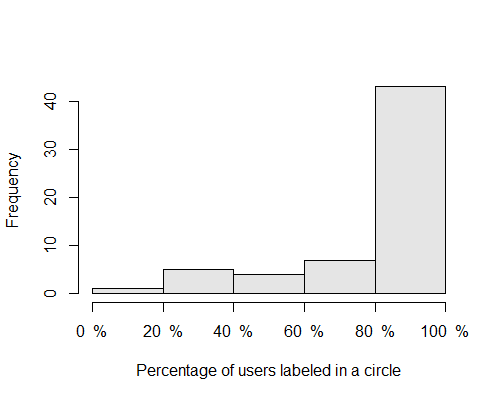
\includegraphics[width=0.9\linewidth]{completecirclelabel.png}
\caption{Distribution of the number of circles per ego}
\end{minipage}
\hspace{0.5cm}
\begin{minipage}[b]{0.47\linewidth}
\centering
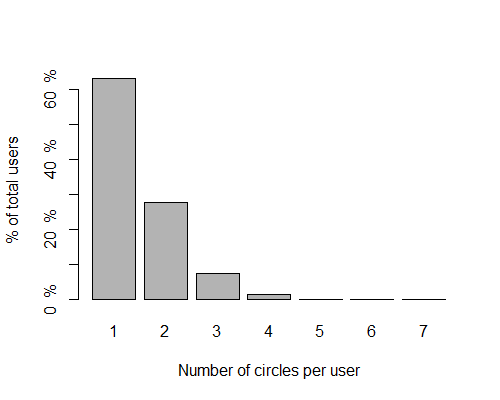
\includegraphics[width=0.9\linewidth]{overlap.png}
\caption{Distribution of the number of users per circle for all networks combined}
\end{minipage}
\end{figure}

\newpage

\section{Community detection methods implemented} \label{communitydetection}

Firstly, the notion of community needs to be precised here. While the literature defines it as group of people living in the same place or sharing common interest, our paper will mainly focus on connection degrees between individuals. This "network thinking" bias is not really far from reality as the intuition leads to think that the more people share common interests, the more likely they will have shared connections (A knowing B  knowing C knowing A for example). 
The first part will be focusing on analysing the network and detecting community with the assumption that communities are formed solely by connections between alters, i.e regardless of the features. We will perform 4 algorithms: leading eigenvector, walktrap, MCL (Markov Clustering Algorithm) and hierarchical clustering. While the second part will take into account the features of each alters by putting a weight on each edge, the weight representing a features-based similarity measure.

\subsection{Leading Eigenvector}
The methodology developed by Mark Newman \cite{Leading_eigen_vector}  is based on the analysis of the edges densities of the vertices that compose the network. It assumes that groups have strong communities structure with dense connection between all individuals of a same group. Mathematically, the problem is equivalent to maximizing the benefit function, also called the modularity function. While very effective in its original format, the algorithm has high computational requirement. Mark Newman propose an approach which consist in rewriting the modularity matrix B by using the adjacency matrix A such that:
$$
B_{ij} = A_{ij} - P_{ij} \\
$$
\emph {where $A_{ij}$ the adjacency matrix of the network\\and $P_{ij}$ is the probability of a connection between two vertices i and j\\\\}
Then calculate the eigen vectors $u$, take the most positive one $u_{max}$, and look at the sign of the components of $u_{max}$ which should be a mix of positive and negative number forming two groups that form two communities. Formerly, given $s$ an index vector with $\mid s \mid = n$, number of vertex, the modularity is maximal for $s$ parallel to $u_{max}$ eigen vector of B and we have : 
$$
s_{i} = \left\{
    \begin{array}{ll}
        {+1} & \mbox{if corresponding element in } u_{max}  \ge 0 \\
        {-1} & \mbox{if corresponding element in } u_{max}  < 0 
    \end{array}
\right.
$$
\\
Zhang propose the following algorithm \cite{Leading_eigen_vector_community}:
\begin{center}
\fbox
{\parbox{10cm}{
Given modularity matrix Q
\begin{enumerate}
\item Compute the leading eigenvector of B.
\item Compute the index vector s and the modularity matrix Q
\item Repeat until Q is stable, subdivise into group otherwise
\end{enumerate}
}}
\end{center}

Community detection rendering on a sample network:
\begin{figure}[H]
\centering
\begin{minipage}[b]{0.47\linewidth}
\vspace{0pt}
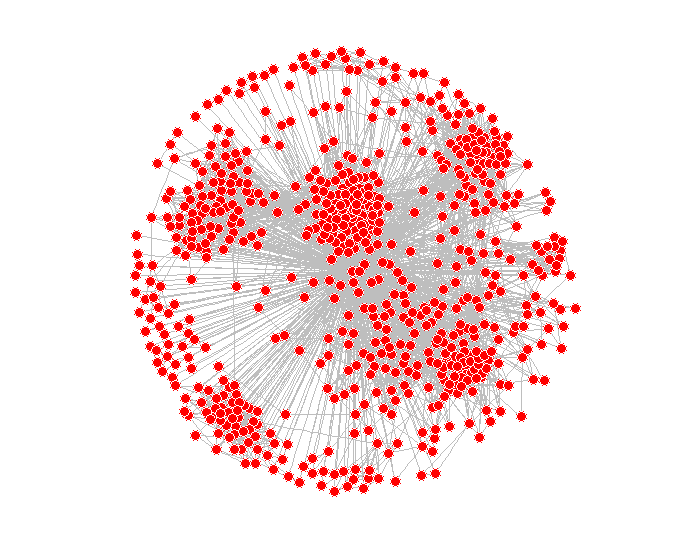
\includegraphics[width=0.9\linewidth]{zNetwork.PNG}
\caption{Original network without any grouping}
\end{minipage}
\hspace{0.5cm}
\begin{minipage}[b]{0.47\linewidth}
\centering
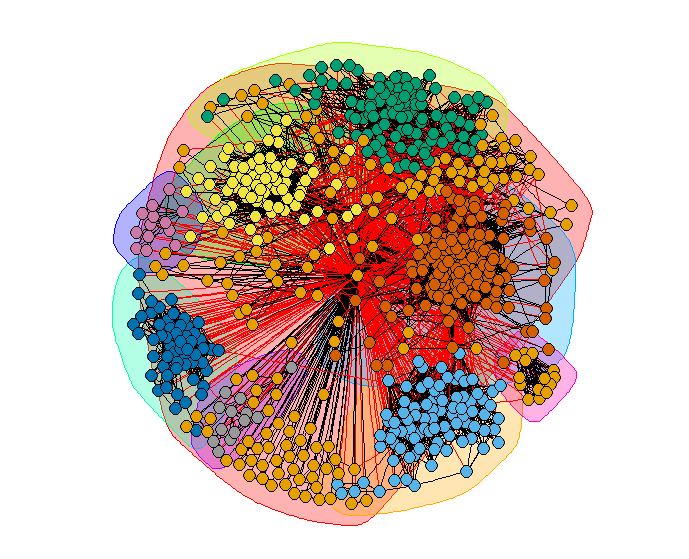
\includegraphics[width=0.9\linewidth]{zNetworkLeadingEV.PNG}
\caption{Leading eigen vector - 7 groups detected}
\end{minipage}
\end{figure}
\captionsetup{type=table}
\begin{center}
\begin{tabular}[b]{rr}
  \hline
 & Values \\ 
  \hline
  Vertices & 670 \\ 
   Edges & 8556 \\
  Communities & 7 \\ 
  True communities & 21 \\ 
   \hline
\end{tabular}
\vspace{0cm}
\caption{Summary of grouping results}
\end{center}
\\
\\
The implementation of the algorithm is done by using the iGraph \textit{leading eigen vector} class which allows us to run a quick, yet precise, test on our sample. The outcome shows us that the grouping is working but the results are too restrained by the number of iteration that it runs, grouping far more communities than the ground truth. Here the true groups are 3 folds the predicted communities. One hypothesis, and as a first step to enhance the precision of the algorithm, is that the communities are abnormally high in this network. (the average is 10, see descriptive statistics part of this paper). Indeed with 21 real groups, we suspect that some communities in the ground truth are in fact nested communities that are not taken into account in the eigen vector methodology. We will confirm that later by looking at the BER which shows far more better results overall. 

\subsection{Walktrap}
The walktrap algorithm has been developed by Matthieu Latapy \cite{Walktrap} and refers the intuition that a random walk in a graph will tend to be trapped in one circle (thus the name walktrap). This methodology, similarly to the previous one assumes that edges between two vertices of a same group are more probable than edges between two vertices from two different communities. Intuitively the edges are "concentrated" within circles.
Latapy calculates the distance between vertices and applies a hierarchical clustering using Ward's agglomeration method to form communities. 
\newline    
Algorithm:
\begin{center}
\fbox
{\parbox{15cm}{
Start with partition $P_{1} = \{\{$v\},$v \in $V \} \newline
Start with n single vertex communities \newline
Compute distance between all adjacent vertices \newline
iterate
\begin{enumerate}
\item Choose two communities $C_{1}$ and $C_{2}$, calculate distance $r$
\item Merge $C_{3}$ = $C_{1}\cup  C_{2}$ and create new partition $P_{k}$ = ($P_{k+1}$ / \{$C_{1}$,$C_{2}\})$ $\cup$  $C_{3}$
\item Update existing distance between communities
\end{enumerate}
}}
\end{center}
\newline
Community detection rendering on a sample network:
\begin{figure}[H]
\centering
\begin{minipage}[b]{0.47\linewidth}
\vspace{0pt}
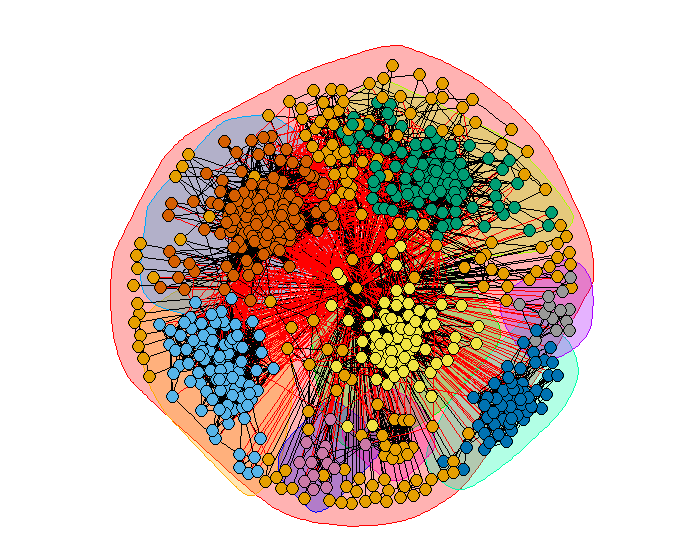
\includegraphics[width=\linewidth]{zNetworkWalktrap.PNG}
\caption{Walktrap algorithm applied to \textit{Figure 16}}
\end{minipage}
\hspace{0.5cm}
\begin{minipage}[b]{0.45\linewidth}
\captionsetup{type=table}
\centering

\begin{tabular}[b]{rr}
  \hline
 & Values \\ 
  \hline
  Vertices & 670 \\
   Edges & 8556 \\
  Communities & 30 \\ 
  True communities & 21 \\ 
   \hline
\end{tabular}
\vspace{2cm}
\caption{Walktrap grouping results}
\end{minipage}
\end{figure}
\newline
The first remark is that the distance used in the algorithm seems rather suitable for community detection. Compared to leading eigen vector we have more granularity in the number of community detected. 
\subsection{MCL}
The Markov cluster algorithm has been developed by Dongen (2000) \cite{MCL}. The methodology is to simulate a random walk using Markov matrices and applying two operators alternatively namely the inflation and the expansion operators. While the former is similar to taking the power of the Markov matrix, the latter uses the scaled Hadamard power of the matrix to obtain a new stochastic matrix. After n iterations the matrix eventually reach a state where it doesn't change neither with expansion nor inflation steps.
The algorithm induce using knowing the network, that is using the adjacency matrix as an input:\newline
\begin{center}
\setlength{\fboxsep}{3pt}
\fbox
{\parbox{13cm}{
\text{Given G a graph}\newline
 \text{Set M1 to be the matrix of random walks on G}\newline
   while (change)
\begin{enumerate}
\item M2 =  M1 * M1    
\item M1 = $\gamma$ * M2     
\item change   =  difference(M1, M2)
\end{enumerate}
}}
\end{center}
\newline

Community detection rendering on a sample network:
\begin{figure}[H]
\centering
\begin{minipage}[b]{0.47\linewidth}
\centering
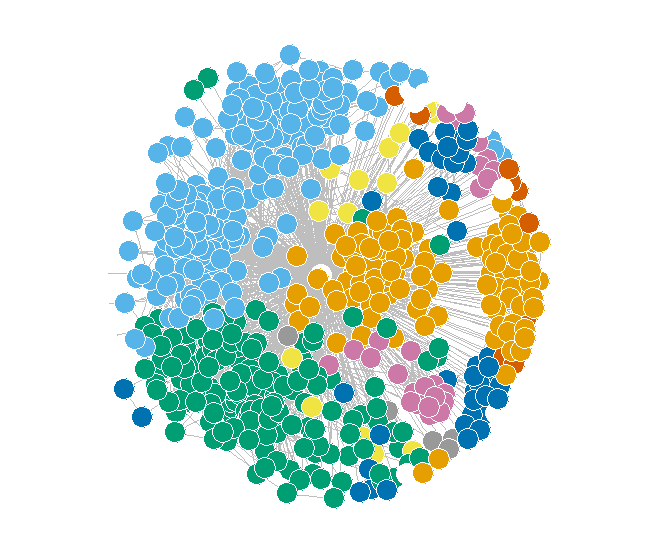
\includegraphics[width=0.9\linewidth]{zNetworkMCL_2.PNG}
\caption{MCL algorithm applied to network \textit{Figure 16}}
\end{minipage}
\hspace{0.5cm}
\begin{minipage}[b]{0.45\linewidth}
\captionsetup{type=table}
\centering
\begin{tabular}[b]{rr}
  \hline
 & Values \\ 
  \hline
  Vertices & 670 \\ 
   Edges & 8556 \\
  Communities & 2 5\\ 
  True communities & 21 \\ 
   \hline
\end{tabular}
\vspace{2cm}
\caption{Hierarchical clustering grouping results}
\end{minipage}
\end{figure}

\subsection{Hierarchical clustering}
In the following, we use a single-linkage clustering \cite{wikiMCL} which is part of the family of hierarchical clustering method which involves calculating a distance D between each vertices. The idea behind hierarchical clustering is to maximize the inner distance and minimize the outer distance at each step. The single linkage clustering assumes that each vertex is a group of its own at step 1 and then sequentially agglomerate groups in which the distance between two vertices of each group is the minimum. 

Algorithm:

\begin{center}
\setlength{\fboxsep}{3pt}
\fbox
{\parbox{13cm}{
Start with $n$ groups composed of single vertex \newline
Repeat until obtaining one group
\begin{enumerate}
\item Calculate all distances of all vertices' alters
\item Merge groups where distance D between two vertices from different group is minimum
\end{enumerate}
}}
\end{center}

\\
Visually, it is easier to look at the grouping process through a dendrogram.

\begin{figure}[H]
\centering
  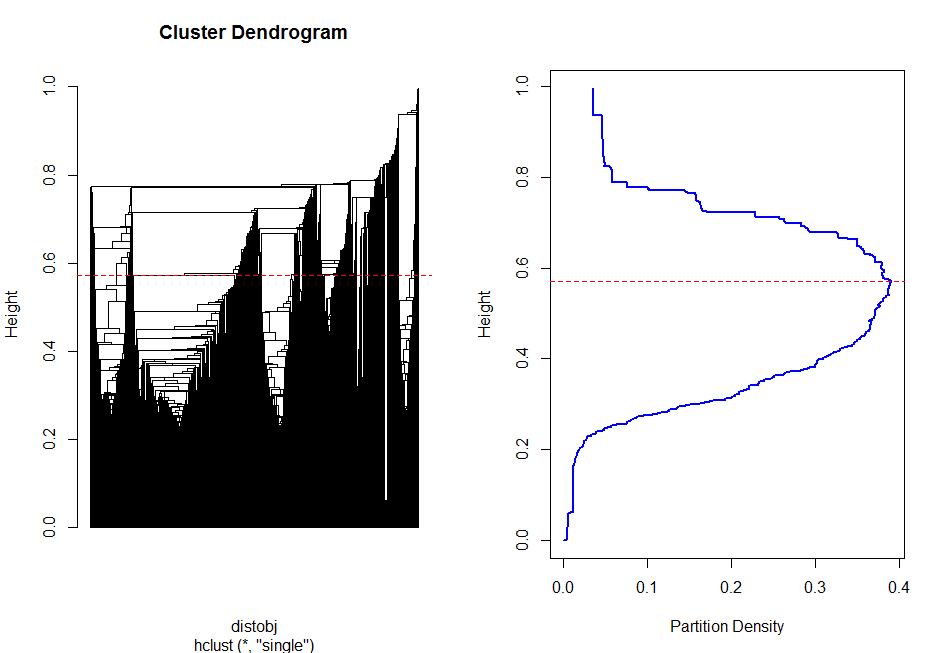
\includegraphics[width=\linewidth]{dendrogramseuil.PNG}
    \caption{dendrogram of single linkage clustering with communities density}
\end{figure}

\begin{figure}[H]
\centering
\begin{minipage}[b]{0.47\linewidth}
\vspace{0pt}
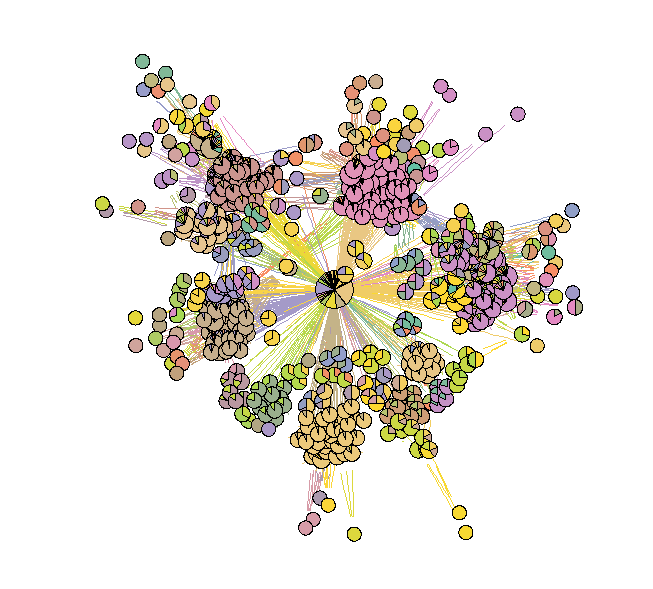
\includegraphics[width=\linewidth]{zNetworkHCnotmerged.PNG}
\caption{Hierarchical clustering algorithm on network \textit{Figure 16}}
\end{minipage}
\hspace{0.5cm}
\begin{minipage}[b]{0.45\linewidth}
\captionsetup{type=table}
\centering
\begin{tabular}[b]{rr}
 \hline
 & Values \\ 
  \hline
  Vertices & 670 \\ 
  Edges & 8556 \\
  Communities & 242 \\ 
  True communities & 21 \\ 
   \hline
\end{tabular}
\vspace{2cm}
\caption{Hierarchical clustering grouping results}
\end{minipage}
\end{figure}


\begin{figure}[H]
\centering
\begin{minipage}[b]{0.47\linewidth}
\vspace{0pt}
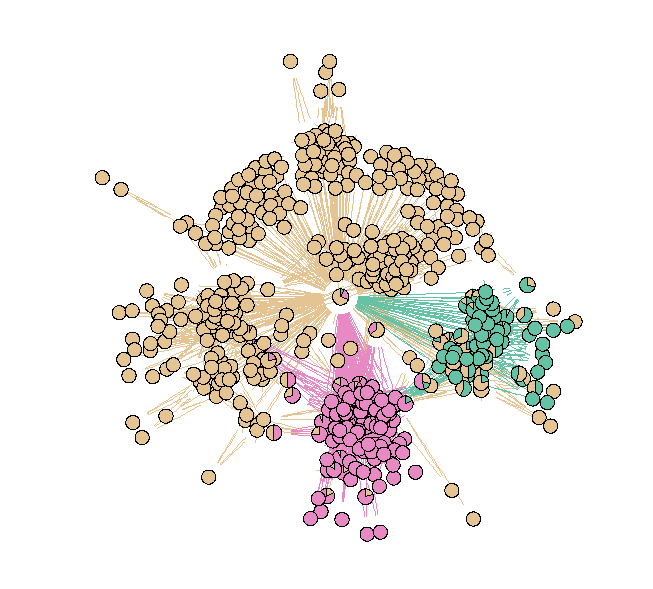
\includegraphics[width=\linewidth]{zNetworkHCmerged.PNG}
\caption{Merging nested communities}
\end{minipage}
\hspace{0.5cm}
\begin{minipage}[b]{0.45\linewidth}
\captionsetup{type=table}
\centering
\begin{tabular}[b]{rr}
   \hline
 & Values \\ 
  \hline
  Vertices & 670 \\
   Edges & 8556 \\
  Communities & 4 \\ 
  True communities & 21 \\ 
   \hline
\end{tabular}
\vspace{2cm}
\caption{Merging results}
\end{minipage}
\end{figure}

The R package we are using, namely Linkcomm, ease the application of the clustering algorithm to our sample network. One advantage of using the library is that it provides a good illustration of possible nested communities. 
In the example we applied two hierarchical clustering methodologies from the package. As we can see the first one has a very high cutting criteria (\textit{fig. 21}), the number of community is very high and really not representative of reality. The second grouping takes the highest partition density (\textit{fig. 20 & fig. 22}) as cutting criteria. We obtain 4 groups (\textit{tab. 11}).
If look in detail the composition of the groups (\textit{fig. 23}), we can see that the algorithm merges the group by taking into account nested communities, i.e. one vertex belonging to two communities. While this is going to cause large discrepancies in number of communities (4 vs 21), it is more accurate when closing the results to the ground truth data (see BER results in part 4)\newline

\begin{figure}[H]
\centering
  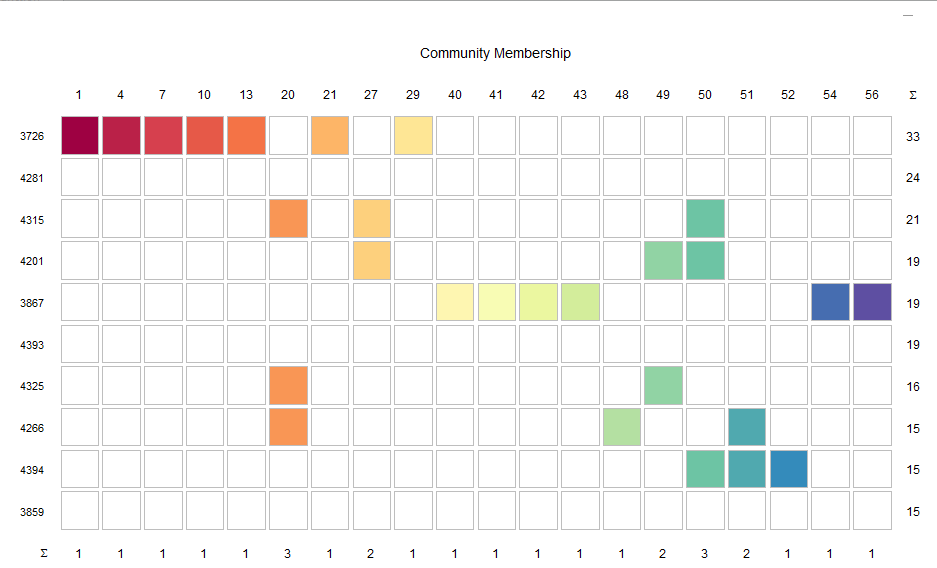
\includegraphics[width=\linewidth]{nested.PNG}
    \caption{Nested communities using Linkcomm hierarchical clustering function \newline\textit{colored cells shows all nodes groups, bottom x-axis is the final group given by the algorithm}}
\end{figure}


\newpage

\subsection{Using profile similarity to compute edge weights}

\begin{table}[H]
\scriptsize
\centering
\begin{tabular}{rccc}
  \hline
 Facebook profile attribute & Vertex 1 & Vertex 2 & Similarity \\ 
  \hline
id & 1 & 146 & FALSE \\ 
  last\_name & 1 & 140 & FALSE \\ 
  first\_name & 1 & 122 & FALSE \\ 
  birthday & 1 & 64 & FALSE \\ 
  name & 1 & 146 & FALSE \\ 
  gender & 1 & 1 & TRUE \\ 
  locale & 0 & 0 & TRUE \\ 
  hometown;id & 1 & 67 & FALSE \\ 
  education;school;id & 0,2,3,3 & 0,86 & TRUE \\ 
  education;type & 0,1,1,1 & 0,1 & TRUE \\ 
  education;year;id & 0,2,3 & 0,10 & TRUE \\ 
  education;concentration;id & 1,2 & 36,70,71 & FALSE \\ 
  location;id & 1 & 0 & FALSE \\ 
  education;classes;from;id & 0 &  & FALSE \\ 
  education;classes;with;id & 0 &  & FALSE \\ 
  education;classes;id & 0 &  & FALSE \\ 
  work;position;id &  & 82 & FALSE \\ 
  work;location;id &  & 33 & FALSE \\ 
  work;start\_date &  & 2 & FALSE \\ 
  work;end\_date &  & 5 & FALSE \\ 
  work;employer;id &  & 132 & FALSE \\ 
  languages;id &  & 2,46 & FALSE \\ 
  work;with;id &  &  & FALSE \\ 
  work;description &  &  & FALSE \\ 
  work;from;id &  &  & FALSE \\ 
   \hline
\end{tabular}
\caption{Illustration of our profile attribute similarity measure for a given edge}
\end{table}

As illustrated in the table\footnote{To simplify the table, we have only represented here a sample of all attributes. All values are represented by integers since our dataset was anonymized. Blank values mean that data is missing.} above, we implemented a very straightforward algorithm to compute our profile attributes similarity and add edge weights to our networks. Our similarity measure for two connected vertices $v_1,v_2$ is defined as:
\begin{equation*}
\textup{Similarity}(v_1,v_2)=\sum_{i=1}^{N_{attr}} \Big{\textbf{1}} \big \{ \textup{attr}_i(v_1) \cap \textup{attr}_i(v_2) \neq \emptyset} \big\}
\end{equation*}

With $\textup{attr}_i$ being the list of past and current values of the $i$-th attribute. It means that if any past or current value of the $i$-th attribute of $v_1$ is the same as that of $v_2$, we add 1 to our similarity measure. For instance, one user could be working at the same company as one of his friends who left the company. Note that we do not count any missing value.\\

Based on this similarity measure, we initialize all weights at 1, and loop over all networks and all edges to add our similarity measure to the weights.



\newpage

\section{Conclusion: Performance evaluation}\label{conclusion}

\subsection{Balanced Error Rate}
In order to compare the implemented methods previously stated, the chosen evaluation metric would be the Balanced Error Rate (BER).

The BER definition in a network-related problem would be as follows :
\begin{equation*}
\displaystyle BER(C_P,C_T) = \frac{1}{2} (\frac{|C_P \setminus C_T|}{|C_P|} + \frac{|C_P^c \setminus C_T^c|}{|C_P^c|})
\end{equation*}

with:
\begin{itemize}
\item $C_P$ : stands for computed circles
\item $C_T$ : stands for ground truth circles
\end{itemize}
\hfill \break

In any given ego-network, we would end up with a ($N_p$ x $N_t$) BER matrix, as for $N_p$ being the number of computed circles and $N_t$ being the number of true circles.\\

Furthermore, as the number of predicted circles are usually not equal to the ground-truth ones, we will have to deal with two cases :
\begin{itemize}
\item{$N_p \leq N_t$ :} the assignment is quite straight forward. For any given predicted circle, the matching true circle would be the one with the maximum (1- BER) rate in any computed line of the BER matrix 
\item{$N_p > N_t$ :} this case leads us to test all merging combinations of computed circles and hence calculate the BER matrix once again. The best combination possible would be the one maximizing the following formula:
\begin{equation*}
\frac{1}{N_t}\displaystyle\sum_{i,j=1}^{N_t}1 - BER(C_m_i,C_t_j)
\end{equation*}
knowing that $C_m_i$ is a computed circle after a merging combination.
\end{itemize}

\subsection{Results}
Here below a synthetic table summing up all results of the community detection methods:

\begin{table}[H]
\centering
\begin{tabular}{c|c|c|}
\cline{2-3}
                                                    & \multicolumn{2}{c|}{\textbf{1 - BER}} \\ \hline
\multicolumn{1}{|c|}{\textbf{Model}}                         & \textbf{Unweighted}   & \textbf{Weighted}  \\ \hline
\multicolumn{1}{|c|}{Leading Eigen Vector}          & 68.9\%       & 69.1\%    \\ \hline
\multicolumn{1}{|c|}{Walktrap}                      & 57.5\%       & 66.2\%    \\ \hline
\multicolumn{1}{|c|}{MCL}                           & 70.7\%       & 70.1\%    \\ \hline
\multicolumn{1}{|c|}{Hierarchical Clustering} & 45.3\%          & 60.9\%       \\ \hline
\end{tabular}
\caption{Comparative performance of the methods implemented}
\end{table}
\newpage

\emph{Evaluation methodology:} Due to the high computational cost of weighting and BER estimation\footnote{In the case where the number of predicted circles is higher than the number of true circles, the complexity becomes exponential as we need to test all merging combinations.}, we have performed this evaluation on a subset of 20 ego-networks, and kept only the giant component. For the Leading Eigenvector and Walktrap methods, we also tuned the parameter controlling for the number of steps in order to avoid predicting too many circles compared to the reality (see subsection \ref{socialcirclelabels}).\\

Comparing all percentages, forgetting at first about the weighted aspect, the MCL algorithm is the one showing the best result (70.7\%). Even though weights are taken into account, the MCL would still be the winner. We notice that the added weights to the ego-networks are not significant enough to either the Leading eigen vector or the MCL, i.e the BER rate is quite similar for the unweighted and the weighted networks.\\

However, for the Walktrap and Hierarchical Clustering, with lower performance, the addition of weights significantly improves the BER. Thus, similarities between the Facebook profiles of two friends can be useful information to detect communities in combination with network data. It can also help interpreting each social circle in terms of shared attributes e.g. employer, school, etc.\\





%% The Appendices part is started with the command \appendix;
%% appendix sections are then done as normal sections
%%\appendix

%%\section{Section in Appendix}
%%\label{appendix-sec1}


%% References
%%
%% Following citation commands can be used in the body text:
%% Usage of \cite is as follows:
%%   \cite{key}         ==>>  [#]
%%   \cite[chap. 2]{key} ==>> [#, chap. 2]
%%

%% References with bibTeX database:

\newpage

\nocite{*}

\bibliography{references}
\bibliographystyle{unsrt}

\end{document}
